\documentclass[10pt,a4paper,titlepage]{report}
\usepackage[utf8]{inputenc}
\usepackage{amsmath}
\usepackage{amsfonts}
\usepackage{amssymb}
\usepackage{graphicx}
\usepackage{xcolor}
\usepackage{minted}

\newcommand{\HRule}[1]{\rule{\linewidth}{#1}}

\nonstopmode


\begin{document}
{\fontfamily{cmr}\selectfont
\title{ \normalsize \textsc{}
\\ [2.0cm]
\HRule{0.5pt} \\
\LARGE \textbf{\uppercase{JOIN STATEMENTS, SET OPERATIONS, NESTED QUERIES AND
GROUPING}
\HRule{2pt} \\ [0.5cm]
\normalsize August 13, 2019 \vspace*{5\baselineskip}}
}

\date{}

\author{
	Rwithik Manoj \\
	College of Engineering, Trivandrum \\
	Department of Computer Science and Engineering }

\maketitle
\newpage

\sectionfont{\scshape}

\subsection*{Tables and their schemas}

\subsubsection{Items}
itemid (primary key) 
itemname 
category
price
instock

\subsubsection{Customers}
custid (primary key)
custname
address
state

\subsubsection{Orders}
orderid (primary key)
itemid
quantity
orderdate

\subsubsection{Delivery}
delivery id (primary key)
custid
orderid

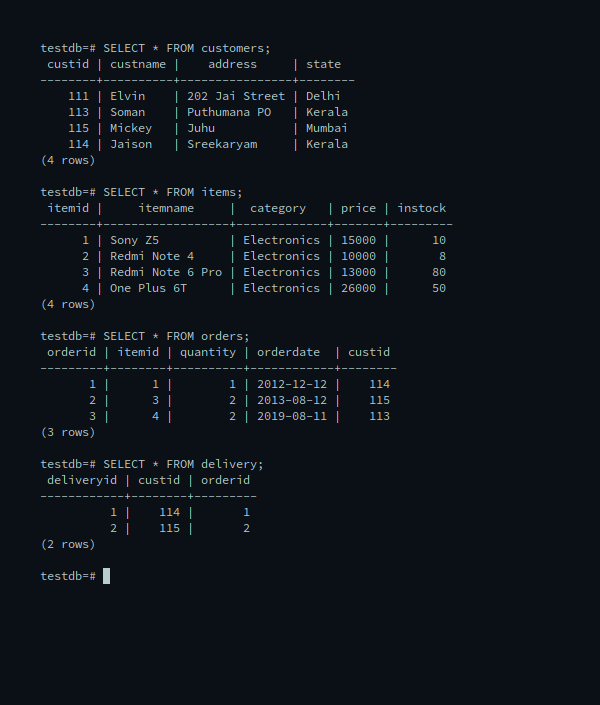
\includegraphics[width=\linewidth]{../Images/Joins/tables.png}

\subsection{Questions}

\begin{enumerate}
	\item List the details of all customers who have placed an order\newline
	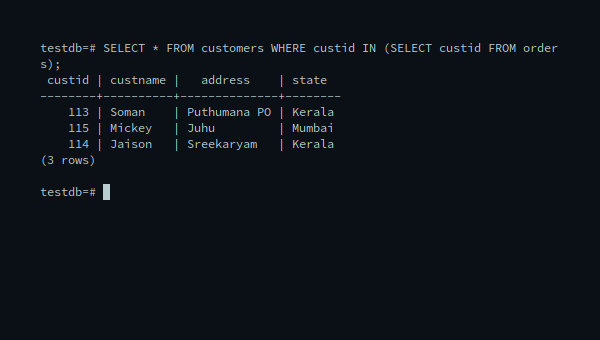
\includegraphics[width=\linewidth]{../Images/Joins/1.png}
	\item List the details of all customers whose orders have been delivered\newline
	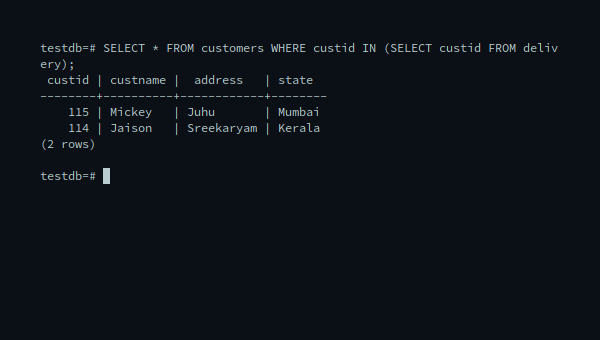
\includegraphics[width=\linewidth]{../Images/Joins/2.png}
	\item Find the orderdate for all customers whose name starts in the letter ‘J’\newline
	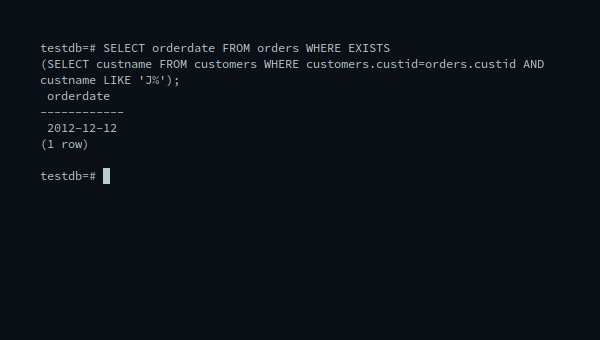
\includegraphics[width=\linewidth]{../Images/Joins/3.png}
	\item Display the name and price of all items bought by the customer ‘Mickey’\newline
	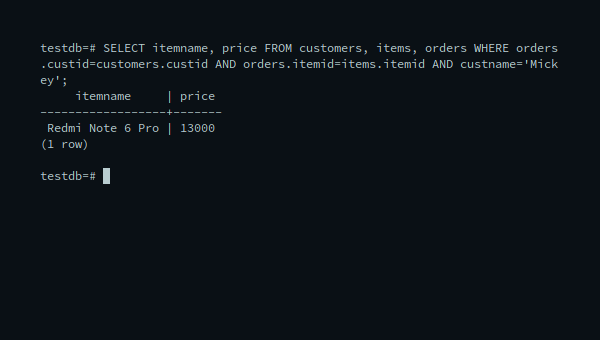
\includegraphics[width=\linewidth]{../Images/Joins/4.png}
	\item List the details of all customers who have placed an order after January 2013 and not received delivery of items.\newline
	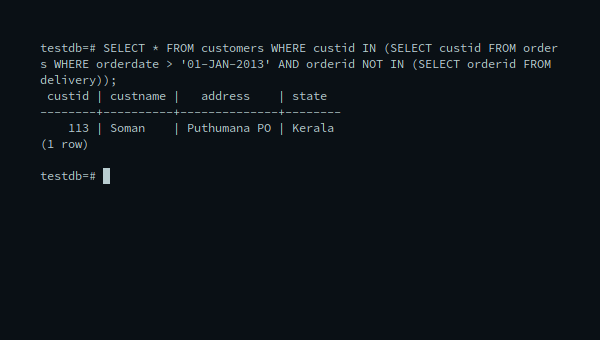
\includegraphics[width=\linewidth]{../Images/Joins/5.png}
	\item Find the itemid of items which has either been ordered or not delivered. (Use UNION)\newline
	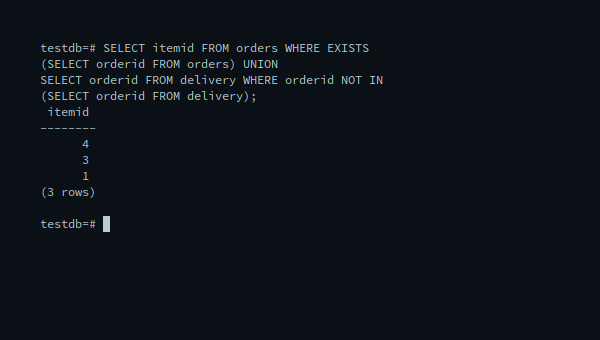
\includegraphics[width=\linewidth]{../Images/Joins/6.png}
	\item Find the name of all customers who have placed an order and have their orders delivered.(Use SET INTERSECTION)\newline
	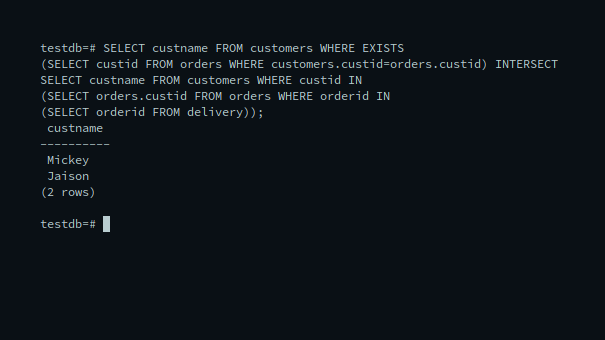
\includegraphics[width=\linewidth]{../Images/Joins/7.png}
	\item Find the custname of all customers who have placed an order but not having their ordersdelivered. (Use SET MINUS)\newline
	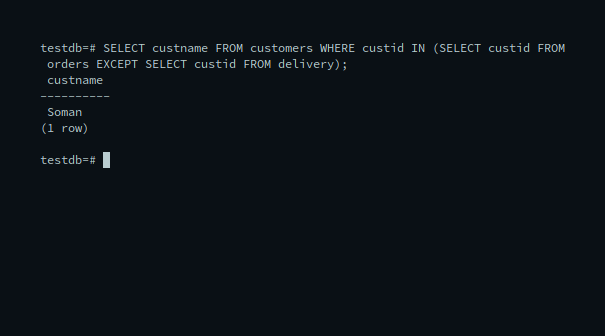
\includegraphics[width=\linewidth]{../Images/Joins/8.png}
	\item Find the name of the customer who has placed the most number of orders.\newline
	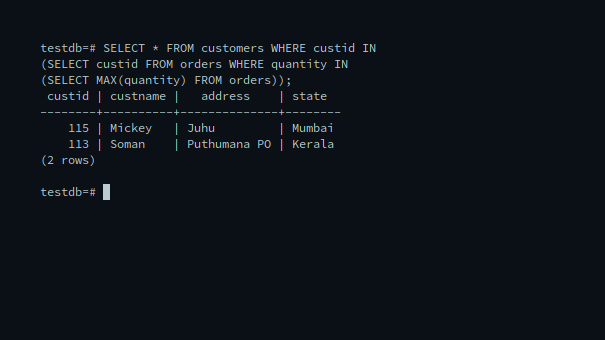
\includegraphics[width=\linewidth]{../Images/Joins/9.png}
	\item Find the details of all customers who have purchased items exceeding a price of 5000\$.\newline
	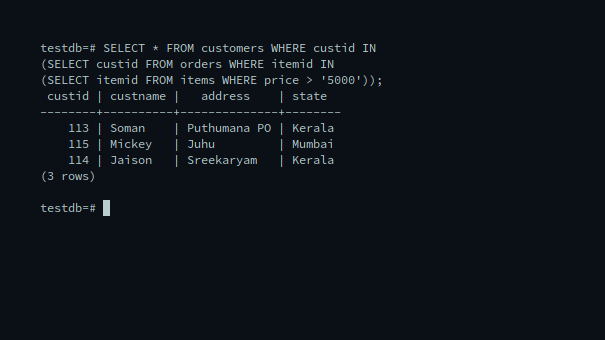
\includegraphics[width=\linewidth]{../Images/Joins/10.png}
	\item Find the name and address of customers who has not ordered a 'Samsung Galaxy S4'\newline
	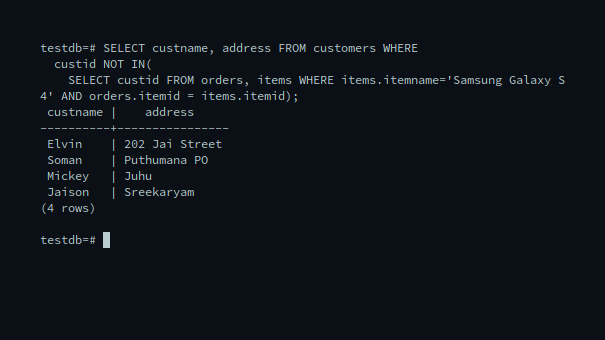
\includegraphics[width=\linewidth]{../Images/Joins/11.png}
	\item Perform Left Outer Join and Right Outer Join on Customers & Orders Table.\newline
	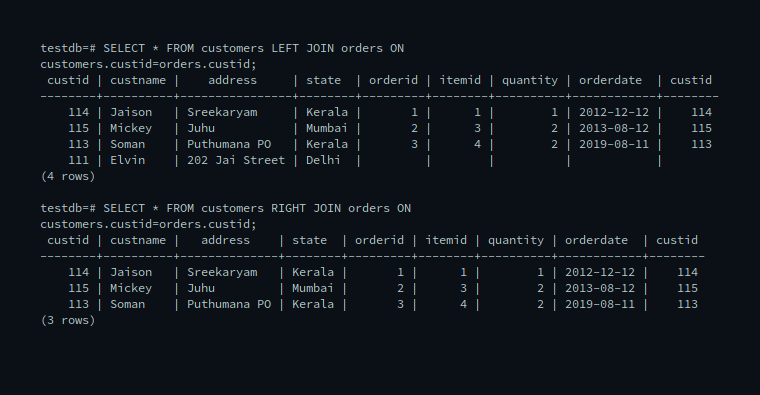
\includegraphics[width=\linewidth]{../Images/Joins/12.png}
	\item Find the details of all customers grouped by state.\newline
	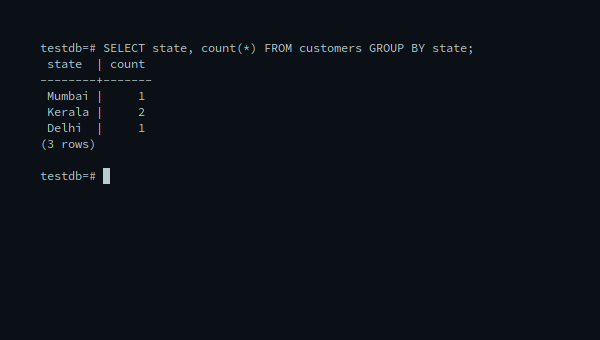
\includegraphics[width=\linewidth]{../Images/Joins/13.png}
	\item Display the details of all items grouped by category and having a price greater than the average price of all items.\newline
	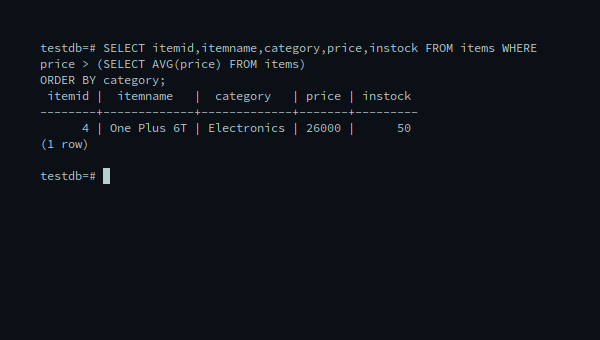
\includegraphics[width=\linewidth]{../Images/Joins/14.png}
\end{enumerate}

\subsubsection*{RESULT}
The query was executed and output was successfully obtained.

}
\end{document}
